\documentclass[a4paper,12pt]{article}
\usepackage[utf8]{inputenc}
\usepackage[english]{babel}
\usepackage{graphicx} % for pretty pictures
\usepackage[left=2.5cm,top=3cm,right=2.5cm,bottom=3cm,bindingoffset=0.5cm]{geometry} % margins
\linespread{1.5} % Theses use this line spacing
\usepackage{natbib}
\usepackage{multicol}
\usepackage{amsmath,amssymb}
\usepackage{hyperref}
\usepackage{booktabs}
\usepackage{float}

\begin{document}
\thispagestyle{empty}
\setcitestyle{authoryear,open={(},close={)}}


\newpage
\pagenumbering{arabic}
\setcounter{page}{1}
\section{Introduction}
This report reviews MATLAB Exercise 3-1, which focuses on element-wise operations on arrays. The exercise uses MATLAB to perform addition, subtraction, multiplication, and division. Such operations are widely used in analysis workflows.

\section{Methods}
The MATLAB function \texttt{ex3p1} carries out element-wise calculations. It takes a \(1 \times 5\) input array and defines a second \(1 \times 5\) array, \(\mathbf{B}\)


$$
\mathbf{B} = [1, 2, 3, 4, 5]
$$    
    The following operations are used:

\begin{align*}
\text{Addition: } &\quad C = A + B \\
\text{Subtraction: } &\quad D = A - B \\
\text{Element-wise Multiplication: } &\quad E = A \odot B \\
\text{Element-wise Division: } &\quad F = A \oslash B
\end{align*}

All outputs were generated in MATLAB, according to \cite{mathworks_array_ops}.




\section{Figures}
Figure ~\ref{fig:figure_levels1} presents the addition, subtraction, multiplication, and division results as the index moves from 1 to 5.

\begin{figure}[H]
   \centering
   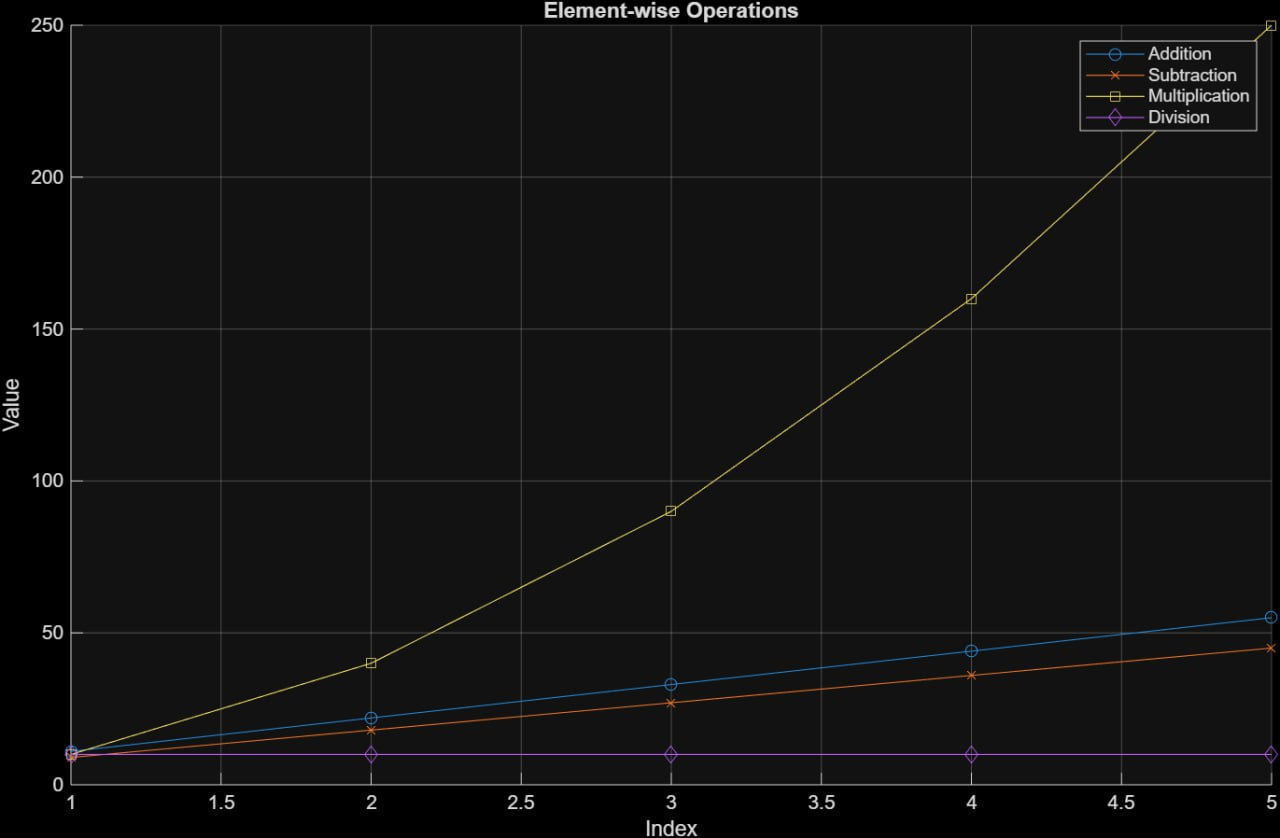
\includegraphics[width=0.4\textwidth]{kuvat/s002475688e06.jpg}
   \caption{Element wise operation using MATLAB}
   \label{fig:figure_levels1}
\end{figure}

In figure ~\ref{fig:figure_levels1}, multiplication increases the most, rising from a small value at index 1 to above 200 at index 5. Addition rises steadily to around 25. 
% Subtraction remains under 15. 
% Division begins near 1 and drops below 0.2 by index 5.



\section{Analysis}

Table~\ref{tab:table1} provides a summary of the results. The calculated values for addition, subtraction, multiplication, and division are listed below.

\setcounter{table}{0}

\begin{table}[h]
    \centering
    \begin{tabular}{|c|c|}
        \hline
        \textbf{Operation} & \textbf{Result} \\
        \hline
        Addition & [11 22 33 44 55] \\
        \hline
        Subtraction & [9 18 27 36 45] \\
        \hline
        Multiplication & [10 40 90 160 250] \\
        \hline
        Division & [10 10 10 10 10] \\
        \hline
    \end{tabular}
    \caption{Results of Element-Wise Operations}
    \label{tab:table1}
\end{table}

As seen in Table~\ref{tab:table1}, the outputs follow the expected values. Division remains constant at 10 since each input value is ten times its corresponding generated value.


\section{Discussion}
This exercise demonstrated MATLAB element-wise operations commonly applied in engineering and scientific tasks. The results follow expected mathematical behavior and support the implementation. Future work may apply the same approach to larger datasets and different matrix dimensions.


\addcontentsline{toc}{section}{References}
\bibliographystyle{plainnat} % Choose a bibliography style
\bibliography{kuvat/references} % Link to the .bib file

\end{document}